\documentclass[twocolumn]{article}
\usepackage[utf8]{inputenc}
\usepackage[T1]{fontenc}
\usepackage[english]{babel}
\usepackage{ifpdf,amsmath,amsthm,amssymb,amsfonts,newtxtext,newtxmath} 
\usepackage{array,graphicx,dcolumn,multirow,hevea,abstract,hanging}
\usepackage[labelfont=sc,textfont=sf]{caption}
\usepackage[hyperfootnotes=false,breaklinks=true]{hyperref}
\urlstyle{rm}
\usepackage[hyphenbreaks]{breakurl}
% DO NOT USE ADDITIONAL PACKAGES unless you make sure they work with Hevea.
% You may define new commands, but these may cause other troubles, so try
% to avoid it.

% FOR BIBTEX USERS (Bibtex is not recommended, but we can use it):
%\usepackage{natbib} % must come afer hyperfootnotes
% insert the following after the \bibliography{} where the references go:
%\bibliographystyle{apalike3}
%\setlength{\bibsep}{0pt}
% replace hyperref above with:
%\usepackage[hyperfootnotes=false,breaklinks=true,linkbordercolor={1 1 1},citebordercolor={1 1 1}]{hyperref}

\usepackage{booktabs} % \toprule \midrule \bottomrule \cmidrule(lr){a-b}
% define centered and ragged columns:
\newcolumntype{L}[1]{>{\raggedright\arraybackslash }p{#1}} % can use m{}
\newcolumntype{C}[1]{>{\centering\arraybackslash }p{#1}}
\newcolumntype{R}[1]{>{\raggedleft\arraybackslash }p{#1}}
\newcolumntype{d}[1]{D{.}{.}{#1}} % d{3.2} for 3 places on l, 2 on r
\newcommand{\mc}{\multicolumn}
\topmargin=-.3in \oddsidemargin=-.1in \evensidemargin=-.1in \textheight=9in \textwidth=6.8in
\setlength\tabcolsep{1mm}
\setlength\columnsep{5mm}
\setlength\abovecaptionskip{.5ex}
\setlength\belowcaptionskip{.5ex}
\setlength\belowbottomsep{.3ex}
\setlength\lightrulewidth{.04em}
\renewcommand\arraystretch{1.2}
\renewcommand{\topfraction}{1}
\renewcommand{\textfraction}{0}
\renewcommand{\floatpagefraction}{.9}
% \renewcommand{\baselinestretch}{1.00} \large\normalsize % for fixing spaces
\widowpenalty=1000
\clubpenalty=1000
\setlength{\parskip}{0ex}
\let\tempone\itemize
\let\temptwo\enditemize
\let\tempthree\enumerate
\let\tempfour\endenumerate
\renewenvironment{itemize}{\tempone\setlength{\itemsep}{0pt}}{\temptwo}
\renewenvironment{enumerate}{\tempthree\setlength{\itemsep}{0pt}}{\tempfour}

%%%%%%%%%%%%%%%%%%%%%%%%%%%%%%%%%%%%%%%%%%%%%%%%%%%%%%%%%%%%%%%%%%%%%
\setcounter{page}{1} % start with first page

\title{How to use this template (and other stuff)}

\author{
Jonathan Baron\thanks{Department of Psychology, University of
  Pennsylvania. Email: baron@upenn.edu.}\;\,\thanks{Some other address.}
\and 
  Some O. Person\thanks{Yet another place.} 
\and
  Y. Another Author\footnotemark[2] % indicates same as 2nd thanks
}


\date{} % leave empty
\begin{document} % goes here

% fill in short title
\newcommand{\jref}{http://journal.sjdm.org/volxx.x.html}
\newcommand{\jhead}{Judgment and Decision Making, Vol.~xx, No.~x}
\newcommand{\jdate}{Month 20xx}
\pagestyle{myheadings} \markright{\protect\small \href{\jref}{\jhead}, \jdate \hfill SHORT TITLE \qquad}
\begin{htmlonly}
\href{\jref}{\jhead}, \jdate, pp.\
\end{htmlonly}
%\begin{latexonly}
\twocolumn[
\vspace{-.3in}
{\small \href{\jref}{\jhead}, \jdate, pp.\ XX--XX}
%\end{latexonly}

\maketitle

%\begin{latexonly}
\vspace{-3mm}
\begin{onecolabstract}
%\end{latexonly}
The abstract is a brief (usually one paragraph) summary
of the whole paper, including the problem, the method for solving
it (when not obvious), the results, and the conclusions suggested
or drawn.  Do not write the abstract as a hasty
afterthought. Look at it as a real exercise in cramming the most
information in one paragraph.  The reader should not have to read
any of the rest of the paper in order to understand the abstract
fully.  Many readers will read only the abstract.  Other readers
will use it to decide what to look for in the paper, or to decide
whether to read the whole thing.  Remember 
\href{http://en.wikipedia.org/wiki/The_Elements_of_Style}{Strunk \&
  White's} admonition, ``Omit needless words.''

\smallskip
\noindent
Keywords: journal, template, latex
%\begin{latexonly}
\end{onecolabstract}\bigskip
]
%\end{latexonly}

{\renewcommand{\thefootnote}{}
\footnotetext{ % note blank lines above and below acknowledgment

  Portions of this template are shamelessly stolen from other
  documents lying around on the author's computer. He is grateful to
  Lenovo, Inc.

Copyright: \copyright\ 2019.
The authors license this article under the terms of the
\href{http://creativecommons.org/licenses/by/3.0/}{Creative Commons
  Attribution 3.0 License.}
}}

\saythanks

\setlength{\baselineskip}{12pt plus.2pt}

\section{Introduction}

To use this file, click ``Open as template''. If you are using EPS graphics (strongly preferred), click on Menu (upper left) and make sure that the compiler is set to LaTeX rather than pdfLaTeX (which used pdf figures).

Here is some meaningless
text as an example. Delete all the text that is not part of your paper.

Einstein said that $E = MC^2$.

Many authors (Jones, 2016; Smith, 2017) have trouble replicating this
result.

Our hypothesis is that $E = MC^3$.

\section{Method} % example of a heading

Here is an example of a one-column table using new column definitions.

%Table 1
\begin{table}[t]
\caption{Experiment 3: Mean (SD) willingness to contribute to identified
and unidentified victims, for self and for the average student.}
\begin{tabular}{L{.7in}C{.7in}C{.7in}C{.7in}}\toprule
 & Self & Average student & Total\\\midrule
Identified victim & 68.28 (55.77) & 45.30 (66.17) & 56.79 (61.89)\\
Unidentified victim & 54.06 (61.89) & 38.63 (67.20) & 46.35 (60.63)\\\midrule
Total & 61.17 (58.81) & 41.97 (66.51) & \\\bottomrule
\mc{4}{p{2.8in}}{Here is a meaningless note about this table.}\\
\end{tabular}
\end{table}

Here is another example of a table (hspace not needed but can be
used). Use ``table*'' with the asterisk when the table needs 2
columns.  A table will generally go at the top of the first page that
refers to it, or as soon after that pages as possible. Do not assume
that tables will appear at the place they are put in the text. In the
tex file, they generally have to go before they are mentioned, in
order to appear in the best place.\footnote{Footnotes at the end of
  sentences should go after the period.}

%Table 2
\begin{table*}[t]\centering
\caption{This table is a very fancy table with a lot of small
  corrections in it, like the tildes in brackets. You don't need to do
this sort of stuff with your own tables. But it may be useful to look
at how notes are done, and how extra space is inserted between columns.}
\begin{tabular}{llrc@{\quad}rc@{\quad}rc@{\quad}rc}\toprule
 &  & \mc{2}{C{1in}}{Accuracy of first response (\%) {\ }} &
\mc{2}{C{1in}}{Accuracy of final response (\%) {\ }} &
\mc{2}{C{1in}}{Change of mind (\%) {\ }} & \mc{2}{C{1in}}{Response time (ms) {\ }}\\
\cmidrule(lr){3-4}\cmidrule(lr){5-6}\cmidrule(lr){7-8}\cmidrule(lr){9-10}
 &  & { ~ } \itshape M & \itshape SD & { ~ }  \itshape M & \itshape SD & { ~ }  \itshape M &
\itshape SD & { ~ ~ }  \itshape M {\ } & \itshape SD\\\midrule
Experiment 1 & Congruent & 73 & 44 & 85 & 36 & 20 & 40 & 1479 & 495\\
 & Incongruent & 45 & 50 & 84 & 37 & 45 & 50 & 1625 & 498\\
Experiment 2 & Congruent & 69 & 46 & 85 & 36 & 26 & 44 & 1567 & 477\\
 & Incongruent & 43 & 50 & 85 & 35 & 49 & 50 & 1695 & 469\\\bottomrule
\mc{10}{p{6in}}{Note. Means and standard deviations are calculated based on the
trial level values (ignoring participants).}
\end{tabular}
\end{table*}

\section{Results}

Use subsections and subsubsections etc. freely.

The following is an example of a one-column figure. The caption can be
long, and fully describe the figure, even if it is redundant with the text.

\begin{figure}[t!]
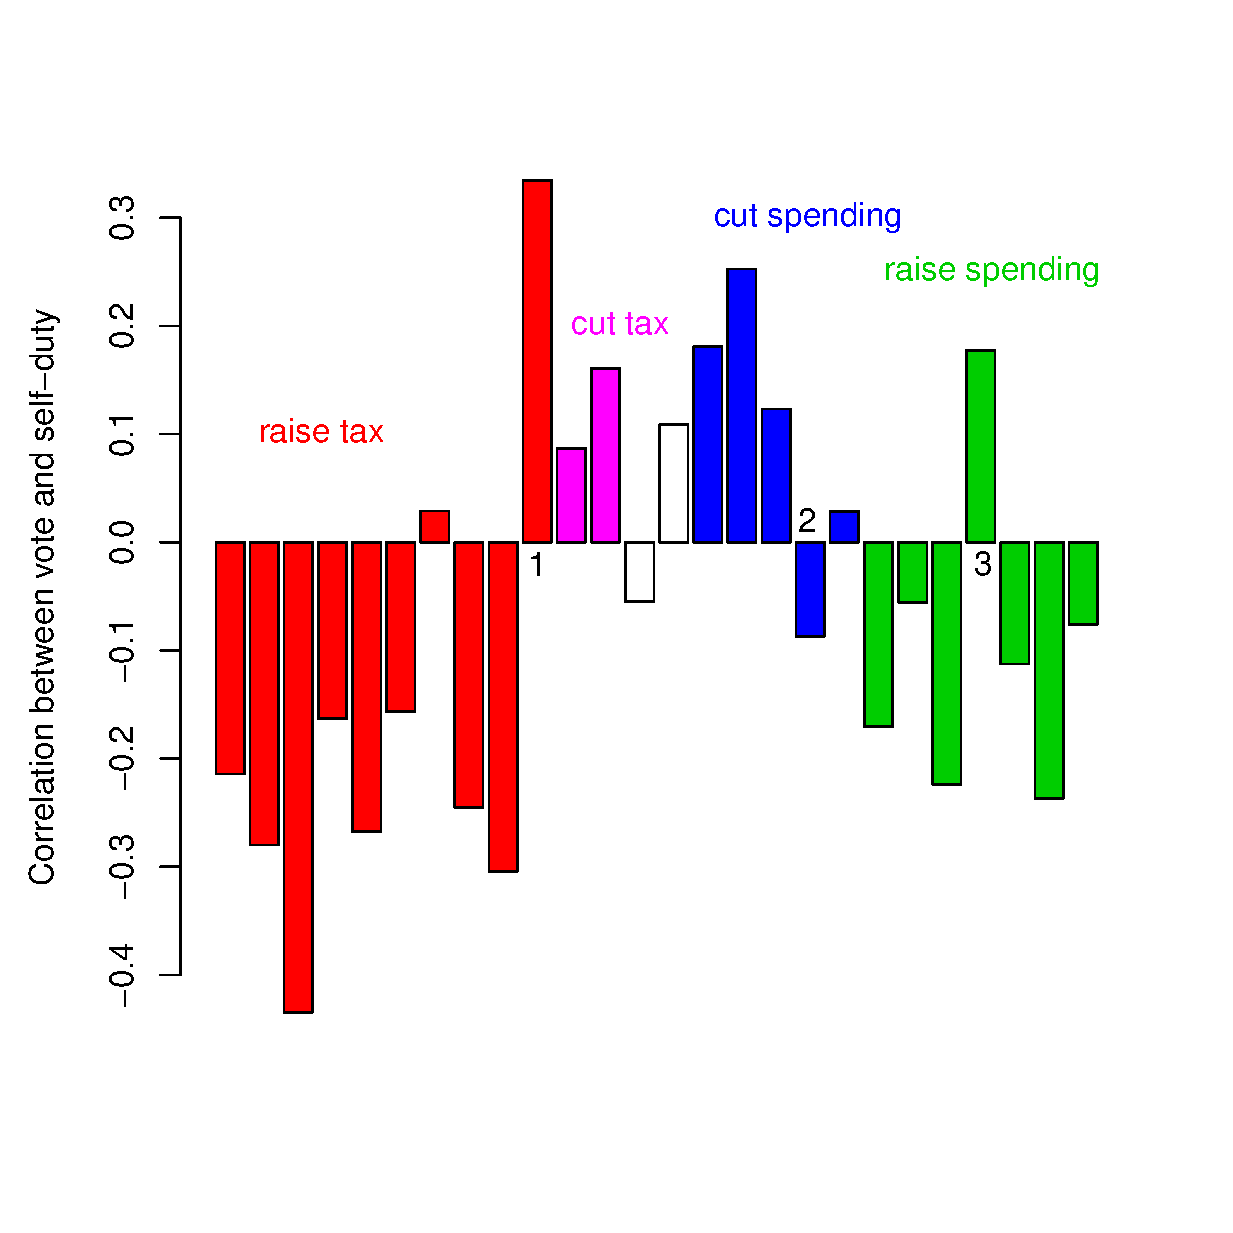
\includegraphics[width=\columnwidth]{dut11.eps}
\caption{The caption goes under the figure like this. Note that
  columnwidth is the width of a column. But you can use any units,
  e.g., ``3in'' or ``50mm''.}
\end{figure}

Here is a two-column figure. A figure will generally go at the top of
the first page that refers to it, or as soon after that pages as
possible. Do not assume that figures will appear at the place they are
put in the text. In the tex file, they generally have to go before
they are mentioned, in order to appear in the best place.

\begin{figure*}[t!]\centering
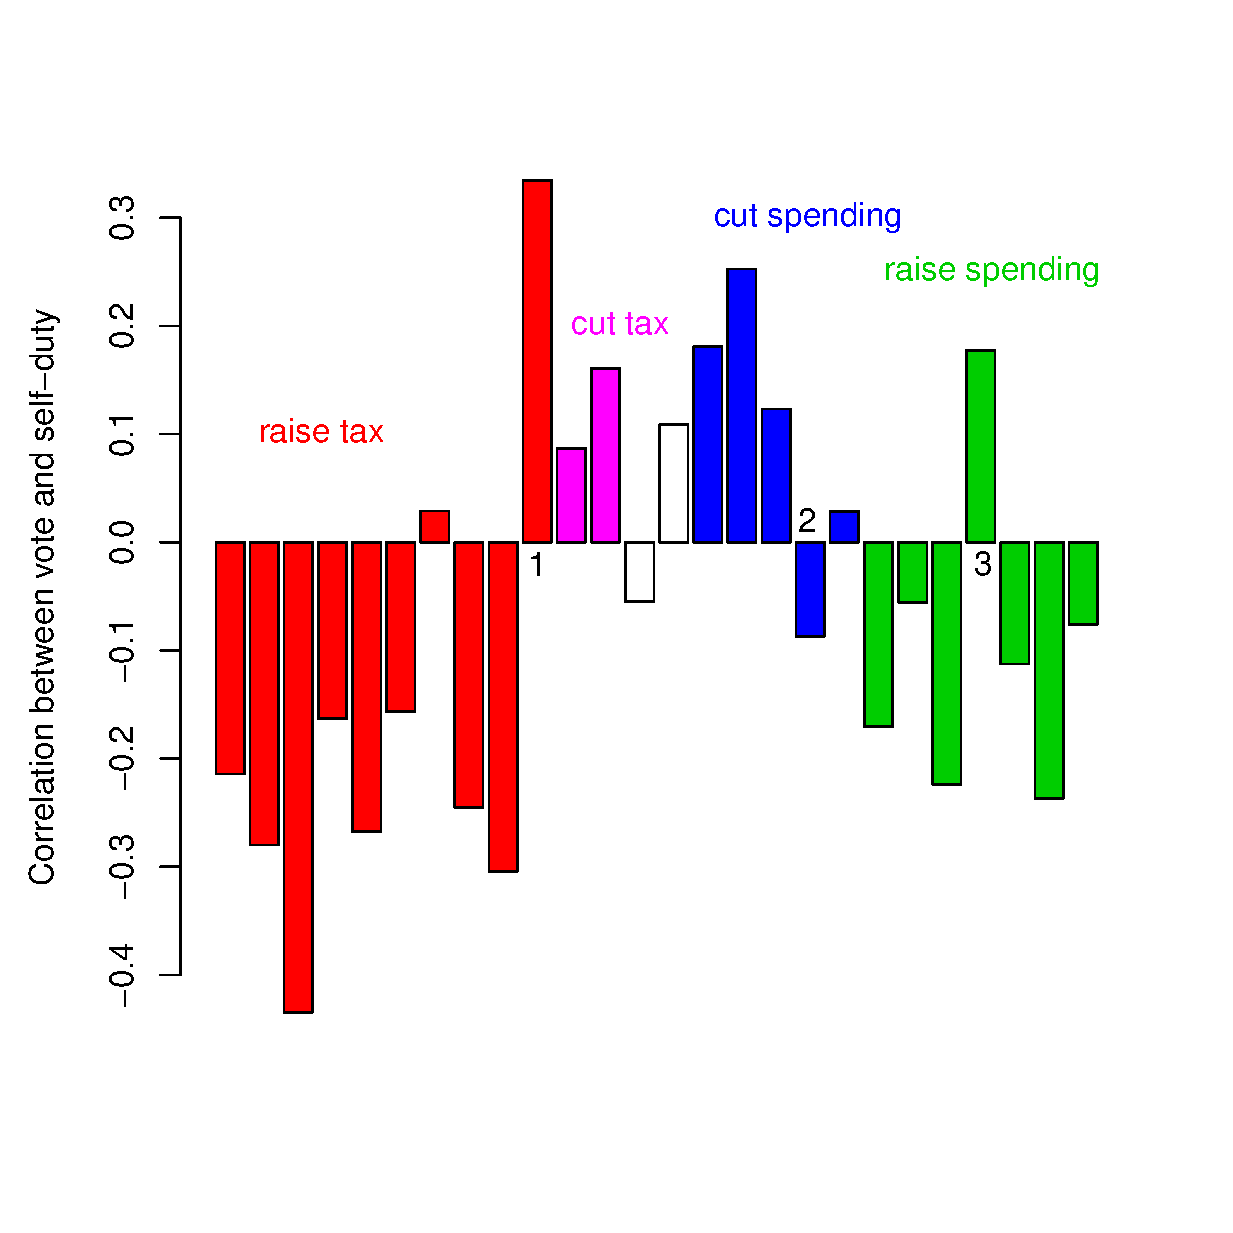
\includegraphics[width=5in]{dut11.eps}
\caption{The caption like this.}
\end{figure*}

\section{Discussion}

It turns out that $E = MC^2$.  Specifically,
\begin{equation}
E = \frac { \sum_{i=1}^n ( M_i C )^2 }{ \alpha + \beta }
\end{equation}
Equation 1 is true.

\subsection{How to write Mathematics}

\LaTeX{} is great at typesetting mathematics. Let $X_1, X_2, \ldots,
X_n$ be a sequence of independent and identically distributed random
variables with $\text{E}[X_i] = \mu$ and $\text{Var}[X_i] = \sigma^2 <
\infty$, and let
\[S_n = \frac{X_1 + X_2 + \cdots + X_n}{n}
      = \frac{1}{n}\sum_{i}^{n} X_i\]
denote their mean. Then as $n$ approaches infinity, the random
variables $\sqrt{n}(S_n - \mu)$ converge in distribution to a normal
$\mathcal{N}(0, \sigma^2)$.

\subsection{How to add Lists}

You can make lists with automatic numbering \dots

\begin{enumerate}
\item Like this,
\item and like this.
\end{enumerate}
\dots or bullet points \dots
\begin{itemize}
\item Like this,
\item and like this.
\end{itemize}

References should be in APA style. Examples are below.

\section*{References}

\begin{hangparas}{1em}{1}

  Aarts, H., \& Dijksterhuis, A. (1999).  How often did I do it?
  Experienced ease of retrieval and frequency estimates of past
  behavior.  \textit{Acta Psychologica, 103}(3), 77--89. \url{http://someurl.html}.

  Barberis, N. \& Thaler, R. (2003). A survey of behavioral finance.
  In G. M. Constantinides, M. Harris \& R. Stultz (Eds.),
  \textit{Handbook of the Economics of Finance,} pp.\ 1053--1123.
  Elsevier Science, North Holland, Amsterdam

\vfill % use this for column breaks
\break

Grice, H. P. (1975).  Logic and conversation. In P. Cole \& J.
L. Morgan, (Eds.), \textit{Speech Acts}, pp.\ 41--58. London: Academic
Press. \url{http://dx.doi.org/3.14159--1x}.
\end{hangparas}

\bigskip
\section*{Appendix}

The asterisk means that these divisions are not numbered.

\subsection*{How to write Mathematics}

This section is completely redundant with the text. Do not do
that. This is just an example.

\LaTeX{} is great at typesetting mathematics. Let $X_1, X_2, \ldots, X_n$ be a sequence of independent and identically distributed random variables with $\text{E}[X_i] = \mu$ and $\text{Var}[X_i] = \sigma^2 < \infty$, and let
\[S_n = \frac{X_1 + X_2 + \cdots + X_n}{n}
      = \frac{1}{n}\sum_{i}^{n} X_i\]
denote their mean. Then as $n$ approaches infinity, the random variables $\sqrt{n}(S_n - \mu)$ converge in distribution to a normal $\mathcal{N}(0, \sigma^2)$.


\subsection*{How to create Sections and Subsections}

Use section and subsections to organize your document. Simply use the section and subsection buttons in the toolbar to create them, and we'll handle all the formatting and numbering automatically.

\end{document}
